\subsubsection{09.12.14}

\begin{enumerate}
	\item The time of beginning and ending of the meeting:
	15:50 - 20:30
	\item Purposes of the meeting:
	\begin{enumerate}
	  \item To strengthen the bucket by superglue.
	  
	  \item To test MOB with the new bucket.
	  
    \end{enumerate}
	\item Work that has been done:
	\begin{enumerate}
	  \item Seams of bucket were fastened by superglue.
	  
	  \item It was turned out that MOB can't turn the bucket because now the length of bucket's lever is 40cm. It impossible to install the sinker due to that MOB is 1cm from maximum height. Now we don't know how to solve this problem but to the next meeting we'll think about it and discuss our ideas.
	  
	  \item By today we bought steel axis with diametr 8mm. It was started replacing of the crossbars. Axis was sawned on pieces with desired length.
	  
	  \item It was decided to make holes in the axis and insert screws in them for fixing it on the lift.
	  
	  \begin{figure}[H]
	  	\begin{minipage}[h]{0.2\linewidth}
	  		\center  
	  	\end{minipage}
	  	\begin{minipage}[h]{0.6\linewidth}
	  		\center{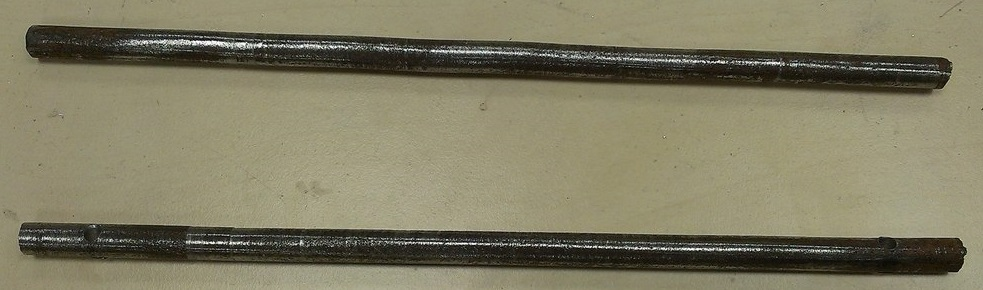
\includegraphics[scale=0.3]{days/09.12.14/images/01}}
	  		\caption{Axis was sawn}
	  	\end{minipage}
	  \end{figure}
      
    \end{enumerate}
    
	\item Results:
	\begin{enumerate}
	  \item The bucket was strengthened by superglue.
	  
	  \item MOB was tested. Now it can't overturn the bucket.
	  
	  \item Steel axis was sawn on the pieces with desired length.
	  
    \end{enumerate}
    
	\item Tasks for the next meetings:
	\begin{enumerate}
	  \item To fix steel crossbars on the lift.
	  
	  \item To solve the problem with overturning the bucket.
	  
    \end{enumerate}     
\end{enumerate}
\fillpage